\chapter{The Multi-Agent Routing and Scheduling through Coalition Formation
Problem}\label{chap:contrib3}

Although many problems similar to the CFSTP have been studied to date (Section
\ref{chap2:limitations}), no one can meet all our research objectives (Section
\ref{sec:objectives}). Against this background, in this final chapter we begin by
presenting in Section \ref{sec:marsc} the \emph{Multi-Agent Routing and Scheduling through
Coalition formation problem} (MARSC), a generalisation of the CFSTP and the TOPTW that can
be used in real-time domains. Then, we define in Section \ref{sec:ant} the first anytime,
exact and parallel MARSC algorithm. Since no exact algorithm has so far been proposed for
the CFSTP, it is consequently the first of its kind for this problem as well. Finally, in
Section \ref{sec:marsc-tests}, using extended versions of the test frameworks of Chapters
\ref{chap:contrib1} and \ref{chap:contrib2}, we evaluate our algorithm on synthetic
small-scale problems, and an approximate variant on large-scale realistic problems.

\section{Problem Formulation}\label{sec:marsc}

As in Section \ref{sec:cfstp-bip}, we use a BIP formulation. Since the MARSC generalises
the CFSTP (Theorem \ref{teo:cfstp-gen}),
we recall and extend the basic definitions and constraints of Sections \ref{sec:defs} $-$
\ref{sec:cv} and \ref{sec:cfstp-bip}.
Specifically, we add multiple possible locations per task, benefits, time windows,
precedences, and define a more general objective function.
We also show how to extend the work of Section \ref{sec:reduction} to reduce the MARSC to
a DynDCOP.

\subsection{Basic Definitions}\label{sec:marsc-defs}

Let $V = \{ v_1, \dots, v_m \}$ be a set of $m$ tasks and $A = \{ a_1, \dots, a_n \}$ be a
set of $n$ agents. Let $L$ be the finite set of all possible task and agent locations.
Time is denoted by $t \in \mathbb{N}$, starting at $t = 0$, and agents travel or perform
tasks with a base time unit of $1$. The time units needed by an agent to travel from one
location to another are given by the function $\rho : A \times L \times L \rightarrow
\mathbb{N}$. Having $A$ in the domain of $\rho$ allows to characterise different agent
features (e.g., speed or type). Let $l_a^t \in L$ be the location of agent $a$ at time
$t$, where $l_a^0$ is the initial location of $a$ and is known a priori.

\paragraph{Task Demand}

Each task $v$ has a \emph{demand} $D_v = (L_v, w_v, \phi_v, \alpha_v, \beta_v, \gamma_v)$,
where:
\begin{itemize}
    \item $L_v \subseteq L$ is the \emph{set of possible locations of} $v$;
    \item $w_v \in \mathbb{R}_{\geq 0}$ is the \emph{workload} of $v$, or the amount of
        work required to complete $v$;
    \item $\phi_v \in \mathbb{R}_{\geq 0}$ is the \emph{benefit} of $v$, or the weight
        associated with the completion of $v$;
    \item $\left[ \alpha_v, \beta_v, \gamma_v \right]$ is the \emph{time window} of $v$,
        such that $\alpha_v \in \mathbb{N}$ is the \emph{earliest time} of $v$, or the
        time starting from which agents can work on $v$, $\beta_v \in \mathbb{N}$ is the
        \emph{soft latest time} of $v$, or the time until which agents can work on $v$
        without incurring in a penalty, and $\gamma_v \in \mathbb{N}$ is the \emph{hard
        latest time} of $v$, or the time until which agents can work on $v$ incurring in a
        penalty. No agent can work on $v$ after $\gamma_v$.
\end{itemize}
We assume that $\alpha_v \leq \beta_v \leq \gamma_v$, $\forall v \in V$, and call $\tmax
=$ $\max_{v \in V} \gamma_v$ the \emph{maximum problem time}.

\paragraph{Task Order}\label{sec:ordering}

Let $Prec \subseteq V \times V$ be such that if $(v_1, v_2) \in Prec$ then $v_1$ must be
completed before $v_2$. Each $(v_1, v_2) \in Prec$ is called a \emph{precedence} and can
be graphically denoted with $v_1 \prec v_2$. As typically done in MRTA
\cite{nunes2017taxonomy}, we assume that $G = (V, Prec)$ is a finite, directed and acyclic
graph. Moreover, without loss of generality, we assume that $Prec$ does not contain
relations which can be inferred transitively, that is:
\begin{equation*}
    (v_1, v_2) \in Prec \land (v_2, v_3) \in Prec \Rightarrow (v_1, v_3) \not\in Prec
\end{equation*}

\paragraph{Coalition and Coalition Value}\label{sec:marsc-cv}

A subset of agents $C \subseteq A$ is called a \emph{coalition}. For each coalition, task
and location there is a \emph{coalition value}, given by the function $u : P(A) \times V
\times L \rightarrow \mathbb{R}_{\geq 0}$, where $P(A)$ is the power set of $A$. The
value of $u(C, v, l)$ is the amount of work that coalition $C$ does on task $v$ at
location $l \in L_v$ in one time unit. In other words, when $C$ performs $v$ in $l$,
$u(C, v, l)$ expresses how well the agents in $C$ work together, and the workload $w_v$
decreases by $u(C, v, l)$ at each time.

\subsection{Decision Variables}\label{sec:marsc-ca}

We use the following indicator variables:
\begin{gather}
    \forall v \in V,\, \forall l \in L_v,\, \forall t \in [\alpha_v,
    \gamma_v],\,
    \forall C \subseteq A,\;
    \mx \in \left\{ 0, 1 \right\}\label{eq:mbip0}\\
    \forall v \in V,\, \forall l \in L_v,\; y_{v, l} \in \left\{ 0, 1 \right\}\label{eq:mbip0b}
\end{gather}
where: $\mx = 1$ if task $v$ in location $l$ and at time $t$ is performed by coalition
$C$, and $0$ otherwise; $y_{v, l} = 1$ if task $v$ is completed in location $l$, and $0$
otherwise.

\subsection{Constraints}\label{sec:marsc-constraints}

There are $4$ types of constraints: structural, temporal, spatial and ordering.
%We formalise each below.

\paragraph{Structural Constraints}

Each task can be performed by at most one coalition at each time, and only within its time
window:
\begin{equation}\label{eq:mbip1}
    \forall v \in V,\, \forall l \in L_v,\, \forall t \in [\alpha_v, \gamma_v],\;
    \sum_{C \subseteq A} \mx \leq 1
\end{equation}

\paragraph{Temporal Constraints}

Each task can be performed in at most one location, and no agent can work on it after its
workload has been completed:
\begin{gather}
    \forall v \in V,\; \sum_{l \in L_v} y_{v, l} \leq 1\label{eq:mbip2a}\\
    \forall v \in V,\, \forall l \in L_v,\;
    \left\lceil \sum_{t \in [\alpha_v, \gamma_v]}\, \sum_{C \subseteq A} u(C, v, l)
    \cdot \mx \right\rceil
    = \left\lceil w_v \cdot y_{v, l} \right\rceil\label{eq:mbip2b}
\end{gather}

\paragraph{Spatial Constraints}

An agent cannot work on a task before reaching one of its possible locations. This
identifies two cases: when an agent reaches a task location from its initial location, and
when an agent moves from one task location to another. The first case imposes that, for
each task $v$, location $l \in L_v$ and coalition $C$, the decision variable $\mx$ can be
positive only if all agents in $C$ can reach $l$ at time $t' < t$:
\begin{equation}\label{eq:mbip3}
    \forall v \in V,\, \forall l \in L_v,\, \forall C \subseteq A,\,
    \text{if } \hat{\rho} = \max_{a \in C} \rho(a, l_a^0, l) \geq \alpha_v
    \text{ then }
    \sum_{t \in [\alpha_v, \hat{\rho}]}\, \mx = 0
\end{equation}
The value of $\hat{\rho}$ is the maximum time at which an agent $a \in C$ reaches $l$,
from its initial location at time $t = 0$. Conditional constraints are usually formulated
using auxiliary variables or the Big-M method. However, such approaches further enlarge
the mathematical program or easily cause numerical issues (Section \ref{sec:cfstp-gaps}).
Consequently, in the preprocessing step necessary to create our BIP, we can implement
Equation \ref{eq:mbip3} simply by excluding the variables that must be equal to $0$.
%That is, if $\hat{\rho} \leq \gamma_v$, we only declare the following variables: $\{ \mx
%\}_{t \in [\hat{\rho} + 1, \gamma_v]}$.
The second case requires that if an agent cannot perform two tasks consecutively, then it
can perform at most one:
\begin{equation}\label{eq:mbip4}
    \begin{gathered}
    \forall C_1, C_2 \subseteq A : C_1 \cap C_2 \neq \emptyset,\,
    \forall v_1, v_2 \in V,\, \forall l_1 \in L_{v_1},\, \forall l_2 \in L_{v_2},\\
    \forall t_1 \in [\alpha_1, \gamma_1],\, \forall t_2 \in [\alpha_2, \gamma_2] :
    t_1 + \max_{a \in C_1 \cap C_2} \rho(a, l_1, l_2) \geq t_2,\\
    x_{v_1,\, l_1,\, t_1, C_1} + x_{v_2,\, l_2,\, t_2, C_2} \leq 1
    \end{gathered}
\end{equation}
Hence, coalition $C_2$ can perform task $v_2$ only if all agents in $C_1 \cap C_2$ can
reach location $l_2$ by the hard latest time $\gamma_2$. Equation \ref{eq:mbip4} also
implies that two tasks cannot be performed by the same agent at the same time.
Consequently, coalitions that exist in different locations at the same time are disjoint.
There are no synchronisation constraints \cite{nunes2017taxonomy}. Thus, when a task $v$
in location $l$ is allocated to a coalition $C$, each agent $a \in C$ starts working on
$v$ as soon as it reaches $l$, without waiting for the remaining agents. That is, $v$ is
completed by a temporal sequence of subcoalitions of $C$: $\exists S \subseteq P(C)$ such
that $\forall C' \in S$, $\exists t \in [\alpha_v, \gamma_v]$, $x_{v,\, l,\, t,\, C'} =
1$, where $P(C)$ is the power set of $C$.

\paragraph{Ordering Constraints}

If $v_1 \prec v_2$ then $v_2$ can only be performed after $v_1$:
\begin{equation}\label{eq:mbip5}
    \forall v_1, v_2 \in V,\, \text{if } v_1 \prec v_2 \text{ then }
    \sum_{l_1 \in L_{v_1}} y_{v_1, l_1} \geq \sum_{l_2 \in L_{v_2}} y_{v_2, l_2}
\end{equation}

\subsection{Objective Function}\label{sec:ofmarsc}

Let $\bm{x}$ be a \emph{solution}, that is, a value assignment to all decision variables,
which defines the route and schedule of each agent. For each task $v$ and time $t$, let:
\begin{equation}\label{eq:penalty}
\psi_{v, t} =
\begin{cases}
    1, & \quad\text{if } t \leq \beta_v\\
    1 - \dfrac{t - \beta_v}{\gamma_v - \beta_v + 1}, & \text{ otherwise}
\end{cases}
\end{equation}
be the \emph{penalty} of performing $v$ at $t$, that is, a positive weight that decreases
linearly after $t$ passes $\beta_v$. Let:
\begin{equation}\label{eq:score}
    score(\bm{x}) =
    \sum_{v \in V}\, \sum_{l \in L_v}\, \sum_{t \in [\alpha_v, \gamma_v]}\,
    \sum_{C \subseteq A}\, \phi_v \cdot \psi_{v, t} \cdot \mx
\end{equation}
be the \emph{score} of $\bm{x}$.
The objective of the MARSC is to find a solution that has maximum score and satisfies all
constraints:
\begin{equation}\label{eq:mbip}
    \arg \max_{\bm{x}} score(\bm{x})
    \text{ subject to Equations \ref{eq:mbip0} $-$ \ref{eq:mbip5}}
\end{equation}
Hence, Equation \ref{eq:mbip} maximises the total benefit while minimising the total time
penalty (i.e., the number of tasks that are completed after their soft latest times).
This involves maximising task completion times and minimising coalition sizes.
Consequently, the number of tasks performed at any one time is the largest, and the most
beneficial tasks are prioritised. Ours is a combination of two objective functions
commonly used in MRTA problems \cite[Section $5$]{nunes2017taxonomy}.
Creating all decision variables (Equation \ref{eq:mbip0}) may require to list all
$\mathcal{L}$-tuples over $P(A)$, where $\mathcal{L} = |V| \cdot |L| \cdot
\tmax$. This implies a worst-case time and space complexity of:
\begin{equation}\label{eq:mccc}
    O\left( {\left(2^{|A|}\right)}^{\mathcal{L}} \right) =
    O\left( 2^{|A| \cdot |V| \cdot |L| \cdot \tmax} \right)
\end{equation}
In addition, searching for an optimal solution exhaustively (Equation \ref{eq:mbip}) may
require to list all possible coalition allocations for each possible permutation of $V$,
with a worst-case time complexity of:
\begin{equation}\label{eq:mcomp}
    O \left( |V|! \cdot |L| \cdot 2^{|A|} \cdot \tmax \right)
\end{equation}

\begin{theorem}\label{teo:cfstp-gen}
    The MARSC generalises the CFSTP.
\end{theorem}
\begin{proof}
We refer to the BIP formulation of the CFSTP given in Section \ref{sec:cfstp-bip}.

The CFSTP is a MARSC where tasks have exactly one location, benefits are homogeneous,
there are neither earliest nor soft latest times, and tasks can be completed in any order.
The structural, temporal and spatial constraints are identical. Given a MARSC solution
$\bm{x}$ and a task $v$, if $\mx = 1$, for some $l \in L_v$, $t \in [\alpha_v, \gamma_v]$
and $C \in P(A)$, then $y_{v, l} = 1$. Thus, in the presence of the above-mentioned
simplifications, Equation \ref{eq:mbip} maximises the number of completed tasks, as
required by the objective function of the CFSTP (Equation \ref{eq:bip}).
\end{proof}

\begin{theorem}\label{teo:toptw-gen}
    The MARSC generalises the TOPTW.
\end{theorem}
\begin{proof}
Based on \cite[Section $3.3$]{top2019}, we first describe the TOPTW using our terminology
(Section \ref{sec:marsc-defs}), then we show that it is a special case of the MARSC.

The TOPTW considers a finite set of tasks, each with a non-negative benefit. Each task has
exactly one location and no soft latest time: $|L_v| = 1 \,\land\, \beta_v = \gamma_v$,
$\forall v \in V$. When a task is completed within its time window, its benefit is added
to the total benefit. Between each pair of tasks there is a fixed travel time. There are
an initial task and a final task, both with a benefit of $0$, an earliest time of $0$ and
a soft latest time of $\tmax$. Each route must begin at the location of the initial task
and end at the location of the final task. The objective is to determine $n$ routes, one
for each agent, that maximise the total benefit.

The travel time between tasks $v_i$ and $v_j$ also includes the \emph{service time} at
$v_j$, that is, the time taken by any coalition to complete $v_j$ \cite[Section
$2.2$]{top2019}. Hence, we set $w_v = 1$, $\forall v \in V$, to ensure that each task is
completed in at most $1$ unit of time. Since travel times depend only on task locations,
we exclude $A$ from the domain of $\rho(\cdot)$. Coalitions are singleton, that is, each
$C$ is such that $|C| = 1$. The coalition value function $u(\cdot)$ always returns $1$.

Because each task has exactly one location and coalitions are singleton, we remove the
subscript $l$ from the decision variables and simply use $a$ instead of $C$ to indicate
the coalition that consists of agent $a$. Hence: $x_{v,\, t,\, a} = 1$ if agent $a$ works
on task $v$ at time $t$, and $0$ otherwise; $y_v = 1$ if task $v$ is completed, and $0$
otherwise. Let $v_{start}$ and $v_{end}$ denote the initial and final tasks, respectively.
The structural constraints (Equation \ref{eq:mbip1}) become:
\begin{equation}
    \forall v \in V \setminus \left\{ v_{start}, v_{end} \right\},\,
    \forall t \in [\alpha_v, \beta_v],\;
    \sum_{a \in A} x_{v,\, t,\, a} \leq 1\label{eq:tops}
\end{equation}
Since both coalition values and workloads are unitary, and each task does not have
multiple locations, Equation \ref{eq:tops} already ensures that a task is completed within
its time window by at most one agent. Hence, no temporal constraints (Equations
\ref{eq:mbip2a} and \ref{eq:mbip2b}) are required.

Let $l_{start}$ denote the location of $v_{start}$, and let $l_v$ denote the location of
any other task $v$. The initial location of each agent is $l_{start}$, and the spatial
constraints (Equations \ref{eq:mbip3} and \ref{eq:mbip4}) become:
\begin{equation}
    \forall v \in V,\, \forall a \in A,\,
    \text{if } \lambda = \rho(l_{start}, l_v) \geq \alpha_v \text{ then }
    \sum_{t \in [\alpha_v, \lambda]} x_{v,\, t,\, a} = 0
\end{equation}
\begin{equation}
\begin{gathered}
    \forall v_1, v_2 \in V,\, \forall a \in A,\,
    \forall t_1 \in [\alpha_1, \beta_1],\, \forall t_2 \in [\alpha_2, \beta_2]
    : t_1 + \rho(l_{v_1}, l_{v_2}) \geq t_2,\\
    x_{v_1,\, t_1,\, a} + x_{v_2,\, t_2,\, a} \leq 1
\end{gathered}
\end{equation}
To ensure that each agent schedule starts with $v_{start}$ and ends with $v_{end}$, we
define the set of precedences as follows:
\begin{equation*}
    Prec = \left\{ (v_{start}, v), (v, v_{end}) : v \in V \setminus \left\{ v_{start},
    v_{end} \right\} \right\}
\end{equation*}
The ordering constraints (Equation \ref{eq:mbip5}) become:
\begin{equation}
    \forall v_1, v_2 \in V,\, \text{if } v_1 \prec v_2 \text{ then }
    y_{v_1} \geq y_{v_2}\label{eq:topf}
\end{equation}
The absence of soft latest times means that there can be no time penalties: $\psi_{v,t} =
1$, $\forall v \in V$, $\forall t \leq \tmax$ (Equation \ref{eq:penalty}). Hence, the
objective function (Equation \ref{eq:mbip}) is simplified as follows:
\begin{equation}
    \begin{gathered}
    \arg \max_{\bm{x}} \sum_{v \in V \setminus \{v_{start}, v_{end}\}}\,
    \sum_{t \in [\alpha_v, \beta_v]}\,
    \sum_{a \in A} \phi_v \cdot x_{v,\, t,\, a}\\
    \text{subject to Equations \ref{eq:tops} $-$ \ref{eq:topf}}
    \end{gathered}
    \label{eq:topof}
\end{equation}
\end{proof}

Both the CFSTP and the TOPTW are NP-hard \cite{ramchurn2010cfstp,top2019}, thus the MARSC
is NP-hard as well.
%\clearpage

\subsection{Reduction of the MARSC to a DynDCOP}\label{sec:reduction2}

Given that the MARSC generalises the CFSTP (Theorem \ref{teo:cfstp-gen}), to reduce it to
a DynDCOP, there are two modifications to be made to the work of Section
\ref{sec:reduction}.

Let $V^t_{completed}$ denote the set of tasks that have been completed at time $t$. The
first modification is to include ordering constraints and the possibility of having
multiple possible locations per task by redefining Equation \ref{eq:dyndcop-d} as follows:
\begin{equation}
    \begin{gathered}
    D_i^t = \big\{
        v \in V^t_{allocable} \,|
        \left(\exists v_2 \in V : v_2 \prec v \Rightarrow v_2 \in V^t_{completed} \right)
        \;\land\\ \exists l \in L_v : t + \rho(a_i^t, l_{a_i^t}, l) \leq \gamma_v \big\}
        \cup \left\{ \varnothing \right\}
    \end{gathered}
\end{equation}
Recall that, in propositional logic, $A \Rightarrow B \equiv \neg A \lor B \equiv
\text{if } A \text{ then } B$.
The second change is to include time windows, benefits and penalties by redefining
Equation \ref{eq:costs} as follows:
\begin{equation}\label{eq:costs2}
    f_i^t(d_{i_1}, \dots, d_{i_{h_i}}) = \min_{\bm{x}_i^t}\, - score(\bm{x}_i^t)
\end{equation}
where each $x_{v_i,\, l,\, t,\, C} \in \bm{x}_i^t$ is such that $C$ is a subset of the
agents that control the variables in the scope of $f_i^t$, while $x_{v_i,\, l,\, t,\, C} =
1$ if $d_{i_{h_i}} = v_i$, for each $h_i$-th agent in $C$ and for some $l \in L_{v_i}$,
and $0$ otherwise.
Being an additive function (Equation \ref{eq:score}), the solution score fits naturally
with the characterisation of $f_i^t(\cdot)$. It is multiplied by $-1$ in Equation
\ref{eq:costs2} because we formulate the DynDCOP as a minimisation problem (Equation
\ref{eq:dcop}).

\section{An Anytime, Exact and Parallel MARSC Algorithm}\label{sec:ant}

A trivial way to solve the MARSC would be to implement Equation \ref{eq:mbip} with solvers
such as CPLEX or GLPK. Although this would guarantee anytime and optimal solutions, it
would also take exponential time and space to create the BIP (Equation \ref{eq:mccc}), in
addition to the time to solve it (Equation \ref{eq:mcomp}). This limits this practice to
offline contexts and very small problems. For example, using CPLEX $20.1$ with our HPC
cluster\footnote{\href{https://www.southampton.ac.uk/isolutions/staff/iridis.page}{The
Iridis $5$ Compute Cluster at the University of Southampton}.}, we can solve within hours
problems with superadditive coalition values, uniformly distributed workloads and time
windows, locations based on the taxicab metric, and $dim = |A|\cdot|V|\cdot|L| \leq 30$.
With greater $dim$ values, CPLEX depletes all memory ($187.5$ GB) and crashes. For this
reason, this section presents the \emph{Anytime, exact and parallel Node Traversal} (ANT)
algorithm, which provides the sharp lower bound on the time and space complexity required
to solve the MARSC optimally. We begin by explaining its procedures, then we analyse its
theoretical properties and computational complexity.
%\clearpage

\subsection{Procedures}\label{sec:procedures}

\begin{algorithm}[t]
    \DontPrintSemicolon
    \KwIn{task $v$, location $l \in L_v$, agents $A'$}
    $\Pi_v \gets$ array of all agents in $A'$ that, from their current \textsf{status},
    can reach $l$ by $\gamma_v$\;
    Sort $\Pi_v$ by arrival time to $l$\;
    $\varphi_v \gets 0$ \Comment{\small total workload done on $v$}
    \For{$i \gets 1$; $i \leq |\Pi_v|$; $i \gets i + 1$}{
        $C^\ast \gets$ first $i$ agents in $\Pi_v$\;
        $\lambda_i \gets$ arrival time to $l$ of the $i$-th agent in $\Pi_v$\;
        \eIf{$i + 1 \leq |\Pi_v|$}{
            $\lambda_{i+1} \gets$ arrival time to $l$ of the $(i+1)$-th agent in
            $\Pi_v$\;
        }(\Comment*[h]{\small the $i$-th agent is the last}){
            $\lambda_{i+1} \gets \gamma_v$ \Comment{\small last feasible working time}
        }
        $\varphi_v \gets \varphi_v + (\lambda_{i+1} - \lambda_i) \cdot u(C^\ast,
        v, l)$ \Comment{\small workload done at time $\lambda_{i+1}$}
        \If{$(\gamma_v - \lambda_{i+1}) \cdot u(C^\ast, v, l) \geq w_v -
            \varphi_v$}{
            \Return $\bm{x}_v$ \Comment{\small using $C^\ast$, $v$, and $l$}
        }
    }
    \Return \textsc{nil}\;
    \caption{\textsf{getSingletonSolution}\label{algo:getSingletonSolution}}
\end{algorithm}

\begin{algorithm}[t]
    \DontPrintSemicolon
    \KwIn{incumbent solution $\bm{x}$, task permutation $V^\alpha$, agents $A'$}
    $\bm{x}^\alpha \gets$ empty vector\;
    \For{$v \in V^\alpha$}{
        $\bm{x}_v^\alpha \gets$ \textsc{nil}\;
        \For{$l \in L_v$}{
            $\bm{x}_{v,l}^\alpha \gets$ \textsf{getSingletonSolution($v$, $l$, $A'$)}\;
            $\bm{x}_v^\alpha \gets \arg \max_{\bm{x}' \in \{\bm{x}_{v,l}^\alpha,
            \bm{x}_v^\alpha\}}
            score(\bm{x}')$\;
        }
        \If{$\bm{x}_v^\alpha \neq$ \normalfont{\textsc{nil}}}{
            $\forall a \in A'$, update $a$\textsf{.status} based on $\bm{x}_v^\alpha$\;
        }
    }

    \Return $\arg \max_{\bm{x}' \in \{\bm{x}^\alpha,
    \bm{x}\}} score(\bm{x'})$ \Comment{\small access to $\bm{x}$ is synchronised}
    \caption{\textsf{getSolutionForSchedule}\label{algo:getSolutionForSchedule}}
\end{algorithm}

Given a task $v$, a location $l \in L_v$ and a set of agents $A' \subseteq A$, Algorithm
\ref{algo:getSingletonSolution} defines a coalition $C^\ast \subseteq P(A')$ such that
$|C^\ast|$ is minimum and each agent $a \in C^\ast$ reaches $l$ not only by $\gamma_v$
(line $1$), but also in the shortest possible time (line $2$), which satisfies the spatial
constraints. The \textsf{status} of each agent (line $1$) is set by Algorithm
\ref{algo:getSolutionForSchedule}. When the condition at line $12$ holds, $C^\ast$
satisfies the temporal constraints. Line $13$ returns a singleton solution $\bm{x}_v
\subseteq \bm{x}$ (Section \ref{sec:reduction}). In particular, $\bm{x}_v$ defines the
temporal sequence of subcoalitions of $C^\ast$ that are formed as the agents reach $l$,
thus satisfying the structural constraints.
That is, for each $a \in C^\ast$, $\bm{x}_v$ defines the time interval $i$ during which
$a$ will work on $v$ at $l$, such that $i$ does not violate any constraints, and
$score(\bm{x}_v)$ is maximum; $a$ is considered part of $C^\ast$ from the moment
$\bm{x}_v$ is created until the end of $i$.

Let $\sigma(V)$ denote the set of all permutations of $V$. Algorithm
\ref{algo:getSolutionForSchedule} takes as input a task permutation $V^\alpha \subseteq
\sigma(V)$ and a set of agents $A' \subseteq A$. It defines a solution $\bm{x}^\alpha$ by
finding singleton solutions following the order of $V^\alpha$. For each $v \in V^\alpha$,
the loop at line $4$ finds a location $l \in L_v$ that maximises $score(\bm{x}_v^\alpha)$,
with the convention that $score(\text{\textsc{nil}}) = 0$.
Lines $7$ and $8$ ensure that $\bm{x}^\alpha$ satisfies the structural constraints by
saving, after finding each singleton solution and for each agent $a \in A'$, the last time
$a$ was working, and at which location (i.e., its \textsf{status}).
%This information is used by Algorithm \ref{algo:getSingletonSolution} to define $\Pi_v$.
At line $9$, $\bm{x}$ is maximised synchronously to allow execution in concurrent
environments.

\begin{algorithm}[t]
    \DontPrintSemicolon
    \KwIn{tasks $V$, demands $\{D_v\}_{v \in V}$, order $Prec$, agents $A$}
    $\bm{x} \gets$ empty vector\;
    Sort $V$ by earliest time, while satisfying the ordering constraints
    \Comment{\small initial schedule}
    $\bm{x} \gets$ \textsf{getSolutionForSchedule($\bm{x}$, $V$, $\text{clone}(A)$)}
    \Comment{\small initial incumbent solution}
    \For(\Comment*[h]{\small remaining schedules}){$V^\alpha \in \sigma(V)$}{
        \If{$V^\alpha$ \textnormal{satisfies the ordering constraints}}{
            $\bm{x} \gets$ \textsf{getSolutionForSchedule($\bm{x}$, $V^\alpha$,
            $\text{clone}(A)$)}\;
            \If{$\exists k \leq |V| : \nexists$ \textnormal{solutions for} $k$
                \textnormal{tasks in} $\bm{x}$}{
                \Break
            }
        }
    }
    \Return $\bm{x}$\;
    \caption{ANT\label{algo:ant}}
\end{algorithm}

Algorithm \ref{algo:ant} describes the overall procedure. Lines $2$ and $3$ initialise the
incumbent solution using the \emph{Earliest Deadline First} (EDF) technique, which is
typically used in real-time systems \cite{stankovic2013edf}. Lines $4 - 6$ launch a thread
with an instance of Algorithm \ref{algo:getSolutionForSchedule} for each \emph{schedule}
or permutation of $V$ that satisfies the ordering constraints. At lines $3$ and $6$, $A$
is cloned to avoid interferences between threads. The stopping criterion at line $7$ works
as follows. Let $k$ be the number of tasks performed in the solution found at line $6$,
let $S$ be the set of all schedules investigated so far, and let $\tilde{X}$ be the set of
all solutions found so far. If for each permutation of $k$ tasks $p$ there is a schedule
in $S$ that starts with $p$, and $\tilde{X}$ does not contain a solution involving $k$
tasks, then there can be no solution for $k' \geq k$ tasks. Since $S$ consequently also
contains schedules starting with each permutation of $k'' < k$ tasks, the search can
safely end.

The reason why it is sufficient that, for each $k$-permutation of tasks $p$, $S$ contains
a schedule $s$ \emph{starting} with $p$, is that $s$ has maximum score for subschedule $p$.
In other words, due to Equation \ref{eq:score}, any schedule $s' \neq s$ containing $p$
(in any position) is such that $score(s') \leq score(s)$. Figure \ref{fig:ant-ex}
shows an example of the execution of Algorithm \ref{algo:ant}.

\subsection{Theoretical Properties}\label{sec:ant-properties}

Algorithm \ref{algo:getSingletonSolution} is based on the following lemma.
\begin{lemma}\label{lemma:1}
$\forall a \in A$, $\forall v \in V$, $\forall t \in [\alpha_v, \gamma_v]$, if $\rho(a,
l_a^0, l_v) > t$, then $\nexists v_2 \in V \setminus \{ v \}$ such that:
\begin{equation}
    \exists l_{v_2} \in L_{v_2},\, \exists t_2 \in [\alpha_{v_2},
    \gamma_{v_2}] : t_2 + \rho(a, l_{v_2}, l_v) \leq t
\end{equation}
\end{lemma}
\begin{proof}
If agent $a$ cannot reach location $l_v$ from its initial location $l_a^0$ by time
$t$, then it cannot reach $l_v$ by $t$ even if it would depart from any other location
at time $t' < t$, because each possible route of $a$ always starts at $l_a^0$.
\end{proof}
Hence, if $\rho(a, l_a^0, l_v) > t$, then we can safely exclude each decision variable
$\mx$ such that $a \in C$. This means that only agents that can reach $l_v$ by $\gamma_v$
are able to form feasible coalitions, and only coalitions that can be formed while agents
reach $l_v$ can maximise $score(\bm{x}_v)$, as demonstrated by the following lemma.
\begin{lemma}\label{lemma:2}
    For the input subproblem, Algorithm \ref{algo:getSingletonSolution} is guaranteed to
    converge to an optimal singleton solution.
\end{lemma}
\begin{proof}
Algorithm \ref{algo:getSingletonSolution} finds a coalition of minimum size $C^\ast$ that
reaches $l$ as fast as possible. This maximises the working time of the agents in
$C^\ast$, that is, the number of positive decision variables, and therefore also the score
(Equation \ref{eq:score}).
\end{proof}
\begin{corollary}\label{cor:1}
    For the input schedule, Algorithm \ref{algo:getSolutionForSchedule} is guaranteed to
    converge to an optimal solution.
\end{corollary}
Hence, if we were to perform the tasks according to a given order $V^\alpha$, Algorithm
\ref{algo:getSolutionForSchedule} would find a solution $\bm{x}^\alpha$ with maximum
score, in particular due to lines $4 - 6$ (Section \ref{sec:procedures}). The previous
results lead to the following theorem.
\begin{theorem}\label{teo:exactness}
    Algorithm \ref{algo:ant} is exact.
\end{theorem}
\begin{proof}
Corollary \ref{cor:1} implies that Algorithm \ref{algo:ant} finds an optimal solution to
each possible schedule (line $5$). Hence, we only need to show that the stopping criterion
(line $7$) does not exclude schedules that have to be investigated. This follows from the
discussion in Section \ref{sec:procedures}: if we investigated all schedules involving $k$
tasks, without finding a solution, then the maximum possible number of completed tasks
must be less than $k$, thus there is no need to continue.
\end{proof}
Lastly, Algorithm \ref{algo:ant} is \emph{pleasingly} parallel \cite[Section
$2.1$]{kepner2009} because each possible schedule (line $6$) is investigated in an
independent thread, and anytime since each iteration of the loop at line $4$ updates the
incumbent solution.

\begin{figure}[t]
    \centering
    \begin{adjustbox}{width=.825\textwidth}
        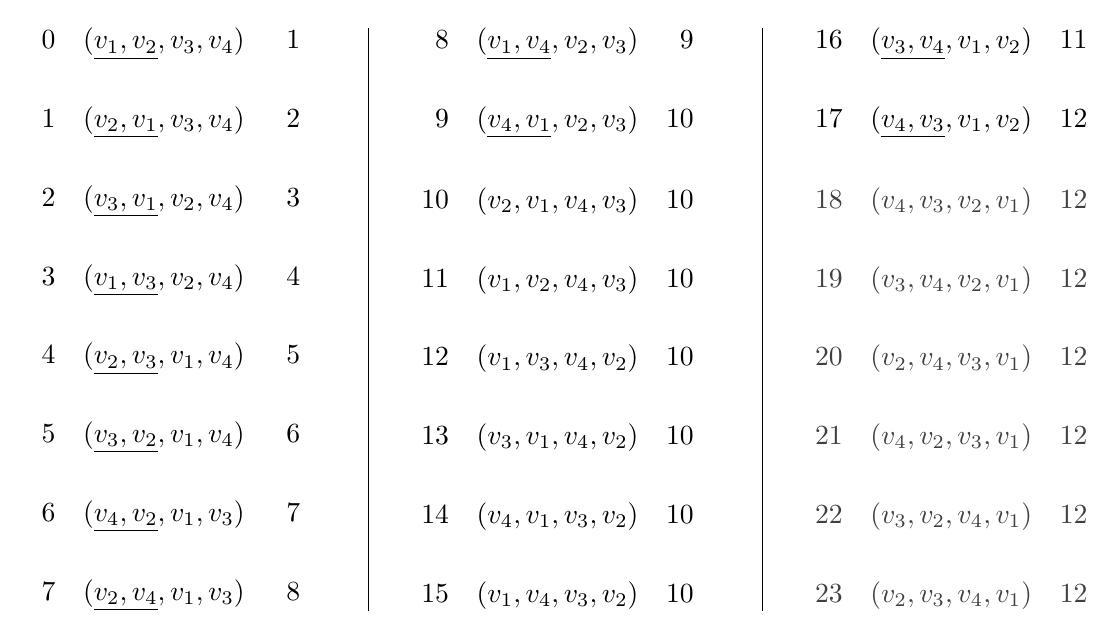
\begin{tikzpicture}
    \node[inner sep=0,outer sep=0] at (0, 8) {$\hphantom{0}0 \quad
        (\underline{v_1, v_2}, v_3, v_4) \quad \hphantom{0}\bm{1}$};
    \node[inner sep=0,outer sep=0] at (0, 7) {$\hphantom{0}1 \quad
        (\underline{v_2, v_1}, v_3, v_4) \quad \hphantom{0}\bm{2}$};
    \node[inner sep=0,outer sep=0] at (0, 6) {$\hphantom{0}2 \quad
        (\underline{v_3, v_1}, v_2, v_4) \quad \hphantom{0}\bm{3}$};
    \node[inner sep=0,outer sep=0] at (0, 5) {$\hphantom{0}3 \quad
        (\underline{v_1, v_3}, v_2, v_4) \quad \hphantom{0}\bm{4}$};
    \node[inner sep=0,outer sep=0] at (0, 4) {$\hphantom{0}4 \quad
        (\underline{v_2, v_3}, v_1, v_4) \quad \hphantom{0}\bm{5}$};
    \node[inner sep=0,outer sep=0] at (0, 3) {$\hphantom{0}5 \quad
        (\underline{v_3, v_2}, v_1, v_4) \quad \hphantom{0}\bm{6}$};
    \node[inner sep=0,outer sep=0] at (0, 2) {$\hphantom{0}6 \quad
        (\underline{v_4, v_2}, v_1, v_3) \quad \hphantom{0}\bm{7}$};
    \node[inner sep=0,outer sep=0] at (0, 1) {$\hphantom{0}7 \quad
        (\underline{v_2, v_4}, v_1, v_3) \quad \hphantom{0}\bm{8}$};

    \node[inner sep=0,outer sep=0] at (5, 8) {$\hphantom{0}8 \quad
        (\underline{v_1, v_4}, v_2, v_3) \quad \hphantom{0}\bm{9}$};
    \node[inner sep=0,outer sep=0] at (5, 7) {$\hphantom{0}9 \quad
        (\underline{v_4, v_1}, v_2, v_3) \quad \bm{10}$};

    \node[inner sep=0,outer sep=0] at (5, 6) {$10 \quad (v_2, v_1, v_4, v_3) \quad 10$};
    \node[inner sep=0,outer sep=0] at (5, 5) {$11 \quad (v_1, v_2, v_4, v_3) \quad 10$};
    \node[inner sep=0,outer sep=0] at (5, 4) {$12 \quad (v_1, v_3, v_4, v_2) \quad 10$};
    \node[inner sep=0,outer sep=0] at (5, 3) {$13 \quad (v_3, v_1, v_4, v_2) \quad 10$};
    \node[inner sep=0,outer sep=0] at (5, 2) {$14 \quad (v_4, v_1, v_3, v_2) \quad 10$};
    \node[inner sep=0,outer sep=0] at (5, 1) {$15 \quad (v_1, v_4, v_3, v_2) \quad 10$};

    \node[inner sep=0,outer sep=0] at (10, 8) {$16 \quad
        (\underline{v_3, v_4}, v_1, v_2) \quad \bm{11}$};
    \node[inner sep=0,outer sep=0] at (10, 7) {$17 \quad
        (\underline{v_4, v_3}, v_1, v_2) \quad \bm{12}$};

    % skipped
    \node[inner sep=0,outer sep=0] at (10, 6) {$\color{darkgray}\sout{18 \quad
        (v_4, v_3, v_2, v_1) \quad 12}$};
    \node[inner sep=0,outer sep=0] at (10, 5) {$\color{darkgray}\sout{19 \quad
        (v_3, v_4, v_2, v_1) \quad 12}$};
    \node[inner sep=0,outer sep=0] at (10, 4) {$\color{darkgray}\sout{20 \quad
        (v_2, v_4, v_3, v_1) \quad 12}$};
    \node[inner sep=0,outer sep=0] at (10, 3) {$\color{darkgray}\sout{21 \quad
        (v_4, v_2, v_3, v_1) \quad 12}$};
    \node[inner sep=0,outer sep=0] at (10, 2) {$\color{darkgray}\sout{22 \quad
        (v_3, v_2, v_4, v_1) \quad 12}$};
    \node[inner sep=0,outer sep=0] at (10, 1) {$\color{darkgray}\sout{23 \quad
        (v_2, v_3, v_4, v_1) \quad 12}$};

    % separators
    \draw (2.6, 8.2) -- (2.6, 0.8);
    \draw (7.6, 8.2) -- (7.6, 0.8);
\end{tikzpicture}

    \end{adjustbox}
    \caption[Illustrative example of the execution of ANT]{%
        Illustrative example of the execution of Algorithm \ref{algo:ant} on a problem
        where $V = \{ v_1, v_2, v_3, v_4 \}$, $Prec = \varnothing$, and $\bm{x}_{v_1}$ is
        the only feasible solution, which is therefore optimal. Each cell of each column
        is an iteration of the loop at line $4$, except the first cell of the first
        column, which represents the initial incumbent solution obtained at line $3$. Each
        cell reports the iteration number, current schedule, and number of schedules
        starting with distinct $2$-permutations of $V$ investigated so far. The schedules
        are generated using Heap's method \cite{sedgewick1977}. Let $\bm{x}_{v_1}$ be
        found at iteration $0$. ANT takes $17$ iterations before ensuring that, for each
        $2$-permutation of $V$ $p$, at least one schedule starting with $p$ has been
        investigated. Thus, the last $6$ schedules ($25\%$ of the total) are skipped.}
    \label{fig:ant-ex}
\end{figure}

\subsection{Computational Complexity}

Algorithm \ref{algo:getSingletonSolution} requires $O(|A| \log |A|)$ time for the sorting
at line $2$ \cite{cormen2009}, and $\bar{a} = O(|A| \cdot (\gamma_v - \alpha_v))$ time and
space to define when each agent $a \in C^\ast$ is working on $v$. Its total time
complexity is $\bar{b} = O(|A| \log |A| \cdot \tmax)$. Algorithm
\ref{algo:getSolutionForSchedule} requires $\bar{c} = O(|V| \cdot |L| \cdot \bar{b})$ time
and $\bar{d} = O(|A| \cdot \tmax)$ space to determine when and where each agent $a \in A$
works, since each variable $y_{v, l}$ can be stored in constant space (e.g., using a
fixed-size string).

Algorithm \ref{algo:ant} requires: $O(|V| \log |V|)$ time and $O(|V|)$ space for line $2$;
$\bar{c}$ time and $\bar{d}$ space for line $3$; $O(|V|!)$ time for the loop at line
$4$, and $O(|V|)$ time for checking the condition at line $5$. The condition at line $7$
can be checked in constant time and space using counter variables. Hence, ANT has an
overall time complexity of:
\begin{equation}\label{eq:ant-tcomp}
    O \left( |V| \log |V| + |V|! \cdot \left( |V| + \bar{c} \right) \right)
    =
    O \left( |V|! \cdot |L| \cdot |A| \log |A| \cdot \tmax \right)
\end{equation}
and an overall space complexity of:
\begin{equation}\label{eq:ant-scomp}
    O \left( |V| + (1 + \kappa) \cdot \bar{d} \right) =
    O \left( |V| + \kappa \cdot |A| \cdot \tmax \right)
\end{equation}
where $\kappa$ is the maximum number of threads available. From Lemma \ref{lemma:1} and
Theorem \ref{teo:exactness}, it follows that no exact MARSC algorithm can have a time and
space complexity lower than that specified by Equations \ref{eq:ant-tcomp} and
\ref{eq:ant-scomp}.
%\clearpage

\section{Empirical Evaluation}\label{sec:marsc-tests}

We wrote a test framework in Java\footnote{\url{https://doi.org/10.5281/zenodo.5375844}}
consisting of two suites. The first is an extension of Section \ref{sec:tests}, while the
second is a variant of Section \ref{sec:dcts-tests} with an extended
dataset\footnote{\url{https://doi.org/10.5281/zenodo.4018139}} of $567492$ task demands
($+67\%$) generated from LFB records of the last $12$ years. We used the first suite to
test ANT on small-scale synthetic problems, and the second suite to test an approximate
variant called ANT-$\varepsilon$ on large-scale realistic problems. This variant simply
limits to $\varepsilon$ the maximum number of iterations done at line $4$ in Algorithm
\ref{algo:ant}. We used Heap's method \cite{sedgewick1977} to generate task
permutations\footnote{In preliminary tests, it proved to be the fastest in finding anytime
solutions among the methods reported in \cite{sedgewick1977}.} in Algorithm
\ref{algo:ant}, and set $\varepsilon = 10^5$. As baselines, we used CTS (Section
\ref{sec:cts}), augmented to solve the MARSC, and EDF\footnote{We use it in place of TOPTW
algorithms, which ignore coalition formation and real-time domains.}, equivalent to lines
$2$ and $3$ of Algorithm \ref{algo:ant}. Below, we detail our test suites and discuss the
results.
\clearpage

\subsection{Setup}

Let $\mathcal{N}$ and $\mathcal{U}$ denote the normal and uniform distribution,
respectively. A test configuration consists of the following base parameters:

\begin{itemize}
    \item $|V| = |A| \cdot k$, where $k \in \{ 1, \dots, 20 \}$;
    \item For each task $v_i$, with $i \leq |V| - 1$, if $\alpha_{v_i} \leq
        \alpha_{v_{i+1}}$ and $\gamma_{v_i} < \gamma_{v_{i+1}}$, then $v_i \prec v_{i+1}$
        has probability $0.5$. That is, the task order is a partial chain defined by coin
        tosses.
\end{itemize}
Each suite then uses the following parameters.

\paragraph{Suite $1$: Synthetic Problems}

\begin{itemize}
    \item $|A| = 2$. Consequently, problems have up to $40$ tasks. From Equation
        \ref{eq:ant-tcomp}, it follows that a problem contains up to $40! \approx 8.16
        \cdot 10^{47}$ schedules to be investigated;
    \item The location space is a $50 \times 50$ grid. $\forall a \in A$, $\forall l_1,
        l_2 \in L$, $\rho(a, l_1, l_2)$ is the Manhattan distance between $l_1$ and $l_2$
        divided by the speed of $a$, which is sampled from $\mathcal{U}(1, 2)$. Each
        agent has a random initial location, while each task has $2$ random possible
        locations;
    \item $\forall v \in V$, $w_v \sim \mathcal{U}(10, 50)$, $\alpha_v \sim \mathcal{U}(5,
        600)$, $\gamma_v \sim \mathcal{U}(\alpha_v, 600)$, $\beta_v \sim
        \mathcal{U}(\alpha_v, \gamma_v)$, and $\phi_v \sim \mathcal{U}(1, 2)$.
\end{itemize}
%\clearpage

\paragraph{Suite $2$: LFB Problems}

\begin{itemize}
    \item Each task demand is defined by a record dated between $1$ January $2009$ and
        $31$ May $2021$ as follows: $\alpha_v = \min_{a \in A} \rho(a, l^0_a, l_v)$;
        $\gamma_v = \alpha_v + \kappa$, where $\kappa$ is the attendance time (in seconds)
        of the firefighters; $\beta_v \sim \mathcal{U}(\alpha_v, \gamma_v)$; $|L_v| = 1$,
        and $\phi_v = 1$. Lastly, since the median attendance time in the whole dataset
        is about $5$ minutes, we set $w_v \sim \mathcal{U}(10, 300)$ to simulate
        wide-ranging workloads;
    \item The remaining parameters are the same as in Section \ref{sec:setup}.
\end{itemize}

\paragraph{Coalition Value Distributions}

We use UC\_NDCS and UC\_Agent-based from Section \ref{sec:setup}, with the following
addition. To simulate real-time domains where the further away $l_v$ is, the lower the
benefit of performing $v$ \cite{stankovic2013edf}, we decrease each $\mu_v = u(C, v, l)$
by $z \sim \mathcal{U}(\mu_v / 10, \mu_v / 4)$ with probability $\rho(\hat{a},
l_{\hat{a}}, l_v) / (\tmax + 1)$, where $\hat{a}$ is the last agent to reach $l_v$, and
$l_{\hat{a}}$ is the location of the task previously completed by $\hat{a}$, or
$l_{\hat{a}}^0$ otherwise. Since it is a touchstone for the study of coalition formation
problems \cite{sandholm1999}, we also use the following special case of Superadditive
distribution: $u(C, v, l) = |C|$.
We ensured consistency between the results of the algorithms as follows. Regarding
Superadditive, all coalition values were computed and stored in hash maps before running
the tests. As it is only defined by coalition sizes, this preprocessing step took $O(|A|)$
time. For UC\_NDCS and UC\_Agent-based, the hash maps were lazy-initialised and shared
among all problems (as done in Section \ref{sec:setup}).

For each test suite, algorithm and coalition value, we solved $100$ problems, and measured
the median and $95\%$ confidence interval of solution score (Equation \ref{eq:score}) and
CPU time\footnote{Based on an Intel Xeon Gold $6138$ ($2$ GHz, $40$ threads).}. Since we
have $3$ algorithms, $20$ task-to-agent ratios, $3$ coalition value distributions, $100$
replicates, and $2$ test suites, the total number of tests performed is $36000$.

\subsection{Results}

\begin{figure}[t]
    \centering
    \begin{adjustbox}{width=\textwidth}
        \begin{tikzpicture}
    \begin{groupplot}[%
        group style={group size=3 by 1, horizontal sep=2cm},
        grid=both,
        grid style={line width=.1pt, draw=gray!10},
        major grid style={line width=.2pt,draw=gray!50},
        xtick={1,4,8,12,16,20},
        ymax=25500,
        every axis plot/.append style={thick},
        legend pos=north west]

        \Large

        \node at (2.27,7.2) {\Large\textsc{Suite $1$: Synthetic Problems $\left( |A| = 2 \right)$}};

        \nextgroupplot [xlabel=$|V| / |A|$,ylabel=$score(\bm{x})$, legend
        entries={\textsc{ant}, \textsc{cts}, \textsc{edf}}, title=(a) Superadditive]

        \addlegendimage{blue,mark=pentagon*,mark options={solid,fill=white}}
        \addlegendimage{green!70!black,mark=diamond*,densely dotted,mark options={solid,fill=white}}
        \addlegendimage{mark=*,red,densely dashed,mark options={solid,fill=red}}

        %% ANT
        \addplot [blue,mark=pentagon*,mark options={solid, fill=white}] plot coordinates {%
            (1, 665)
            (2, 1328)
            (3, 1955)
            (4, 2634)
            (5, 3223)
            (6, 3844)
            (7, 4432)
            (8, 5103)
            (9, 5729)
            (10, 6201)
            (11, 6689)
            (12, 7308)
            (13, 8001)
            (14, 8530)
            (15, 9121)
            (16, 9781)
            (17, 10335)
            (18, 10912)
            (19, 11528)
            (20, 12207)
        };

        \addplot [name path=u2, draw=none] plot coordinates {%
            (1, 657)
            (2, 1370)
            (3, 1998)
            (4, 2692)
            (5, 3282)
            (6, 3918)
            (7, 4565)
            (8, 5203)
            (9, 5807)
            (10, 6322)
            (11, 6793)
            (12, 7441)
            (13, 8074)
            (14, 8637)
            (15, 9295)
            (16, 9882)
            (17, 10444)
            (18, 11069)
            (19, 11651)
            (20, 12365)
        };

        \addplot [name path=l2, draw=none] plot coordinates {%
            (1, 603)
            (2, 1286)
            (3, 1911)
            (4, 2585)
            (5, 3185)
            (6, 3752)
            (7, 4373)
            (8, 5010)
            (9, 5611)
            (10, 6100)
            (11, 6587)
            (12, 7227)
            (13, 7901)
            (14, 8391)
            (15, 9072)
            (16, 9687)
            (17, 10265)
            (18, 10791)
            (19, 11451)
            (20, 12073)
        };

        \addplot+ [fill=blue!15,postaction={pattern color=blue!25, pattern=dots}] fill between[of=u2 and l2];

        %% CTS
        \addplot [green!70!black,mark=diamond*,densely dotted,mark options={solid, fill=white}] plot coordinates {%
            (1, 658)
            (2, 1236)
            (3, 1817)
            (4, 2463)
            (5, 3032)
            (6, 3636)
            (7, 4232)
            (8, 4864)
            (9, 5520)
            (10, 6049)
            (11, 6628)
            (12, 7019)
            (13, 7102)
            (14, 7190)
            (15, 7246)
            (16, 7090)
            (17, 7193)
            (18, 7213)
            (19, 7300)
            (20, 7359)
        };

        \addplot [name path=u2, draw=none] plot coordinates {%
            (1, 689)
            (2, 1274)
            (3, 1872)
            (4, 2518)
            (5, 3091)
            (6, 3730)
            (7, 4322)
            (8, 4968)
            (9, 5620)
            (10, 6145)
            (11, 6770)
            (12, 7179)
            (13, 7238)
            (14, 7357)
            (15, 7446)
            (16, 7461)
            (17, 7347)
            (18, 7430)
            (19, 7448)
            (20, 7564)
        };

        \addplot [name path=l2, draw=none] plot coordinates {%
            (1, 625)
            (2, 1202)
            (3, 1794)
            (4, 2408)
            (5, 2984)
            (6, 3588)
            (7, 4154)
            (8, 4809)
            (9, 5441)
            (10, 5995)
            (11, 6557)
            (12, 6897)
            (13, 6928)
            (14, 6941)
            (15, 7143)
            (16, 6962)
            (17, 7096)
            (18, 7079)
            (19, 6988)
            (20, 7197)
        };

        \addplot+ [fill=green!20,postaction={pattern color=green!35, pattern=north east lines}] fill between[of=u2 and l2];

        %% EDF
        \addplot [dashed, red,mark=*,mark options={solid}] coordinates {%
            (1, 525)
            (2, 941)
            (3, 1303)
            (4, 1642)
            (5, 1905)
            (6, 2168)
            (7, 2325)
            (8, 2401)
            (9, 2481)
            (10, 2502)
            (11, 2493)
            (12, 2515)
            (13, 2558)
            (14, 2548)
            (15, 2530)
            (16, 2529)
            (17, 2534)
            (18, 2506)
            (19, 2527)
            (20, 2528)
        };

        \addplot [name path=u1, draw=none] plot coordinates {%
            (1, 557)
            (2, 970)
            (3, 1340)
            (4, 1682)
            (5, 1939)
            (6, 2203)
            (7, 2382)
            (8, 2471)
            (9, 2535)
            (10, 2570)
            (11, 2544)
            (12, 2559)
            (13, 2616)
            (14, 2605)
            (15, 2581)
            (16, 2597)
            (17, 2603)
            (18, 2574)
            (19, 2587)
            (20, 2615)
        };

        \addplot [name path=l1, draw=none] plot coordinates {%
            (1, 502)
            (2, 919)
            (3, 1259)
            (4, 1599)
            (5, 1881)
            (6, 2114)
            (7, 2260)
            (8, 2354)
            (9, 2449)
            (10, 2455)
            (11, 2446)
            (12, 2455)
            (13, 2522)
            (14, 2489)
            (15, 2476)
            (16, 2462)
            (17, 2497)
            (18, 2460)
            (19, 2492)
            (20, 2493)
        };

        \addplot+ [fill=red!20,postaction={pattern color=red!35, pattern=north
        west lines}] fill between[of=u1 and l1];

        \nextgroupplot[xlabel=$|V| / |A|$,ylabel=$score(\bm{x})$, legend
        entries={\textsc{ant}, \textsc{cts}, \textsc{edf}}, title=(b) UC\_NDCS]

        \addlegendimage{blue,mark=pentagon*,mark options={solid,fill=white}}
        \addlegendimage{green!70!black,mark=diamond*,densely dotted,mark options={solid,fill=white}}
        \addlegendimage{mark=*,red,densely dashed,mark options={solid,fill=red}}

        %% ANT
        \addplot [blue,mark=pentagon*,mark options={solid, fill=white}] plot coordinates {%
            (1, 1340)
            (2, 2630)
            (3, 3479)
            (4, 4362)
            (5, 5305)
            (6, 6399)
            (7, 6688)
            (8, 7512)
            (9, 7910)
            (10, 10387)
            (11, 10783)
            (12, 12823)
            (13, 13140)
            (14, 11731)
            (15, 14330)
            (16, 15972)
            (17, 16986)
            (18, 19052)
            (19, 18082)
            (20, 20622)
        };

        \addplot [name path=u2, draw=none] plot coordinates {%
            (1, 1685)
            (2, 3122)
            (3, 4267)
            (4, 5117)
            (5, 6256)
            (6, 6936)
            (7, 7999)
            (8, 10336)
            (9, 9509)
            (10, 13330)
            (11, 12931)
            (12, 16791)
            (13, 16550)
            (14, 14629)
            (15, 17482)
            (16, 20096)
            (17, 21916)
            (18, 25446)
            (19, 21996)
            (20, 24809)
        };

        \addplot [name path=l2, draw=none] plot coordinates {%
            (1, 1022)
            (2, 1993)
            (3, 2625)
            (4, 4716)
            (5, 4992)
            (6, 5862)
            (7, 6218)
            (8, 6315)
            (9, 6515)
            (10, 7659)
            (11, 9135)
            (12, 9480)
            (13, 10403)
            (14, 10401)
            (15, 12436)
            (16, 13435)
            (17, 13760)
            (18, 14453)
            (19, 14706)
            (20, 17562)
        };

        \addplot+ [fill=blue!15,postaction={pattern color=blue!25, pattern=dots}] fill between[of=u2 and l2];

        %% CTS
        \addplot [green!70!black,mark=diamond*,densely dotted,mark options={solid, fill=white}] plot coordinates {%
            (1, 1200)
            (2, 2407)
            (3, 3421)
            (4, 3886)
            (5, 4451)
            (6, 4551)
            (7, 5557)
            (8, 5420)
            (9, 5224)
            (10, 6300)
            (11, 6318)
            (12, 6139)
            (13, 6566)
            (14, 6644)
            (15, 6655)
            (16, 6496)
            (17, 6440)
            (18, 6067)
            (19, 6313)
            (20, 6290)
        };

        \addplot [name path=u2, draw=none] plot coordinates {%
            (1, 1399)
            (2, 2638)
            (3, 3906)
            (4, 4716)
            (5, 5593)
            (6, 5328)
            (7, 5866)
            (8, 6044)
            (9, 6252)
            (10, 6668)
            (11, 6862)
            (12, 6736)
            (13, 6905)
            (14, 7102)
            (15, 7073)
            (16, 6813)
            (17, 6900)
            (18, 6809)
            (19, 6778)
            (20, 6693)
        };

        \addplot [name path=l2, draw=none] plot coordinates {%
            (1, 881)
            (2, 1843)
            (3, 2591)
            (4, 3396)
            (5, 3975)
            (6, 4096)
            (7, 4554)
            (8, 4464)
            (9, 4666)
            (10, 5681)
            (11, 5372)
            (12, 5284)
            (13, 5958)
            (14, 6098)
            (15, 6268)
            (16, 5706)
            (17, 5485)
            (18, 5342)
            (19, 5796)
            (20, 5587)
        };

        \addplot+ [fill=green!20,postaction={pattern color=green!50, pattern=north east lines}] fill between[of=u2 and l2];

        %% EDF
        \addplot [dashed, red,mark=*,mark options={solid}] coordinates {%
            (1, 794)
            (2, 1283)
            (3, 1677)
            (4, 1995)
            (5, 2164)
            (6, 2236)
            (7, 2281)
            (8, 2280)
            (9, 2278)
            (10, 2283)
            (11, 2329)
            (12, 2308)
            (13, 2336)
            (14, 2303)
            (15, 2318)
            (16, 2333)
            (17, 2332)
            (18, 2343)
            (19, 2342)
            (20, 2313)
        };

        \addplot [name path=u1, draw=none] plot coordinates {%
            (1, 952)
            (2, 1392)
            (3, 1800)
            (4, 2050)
            (5, 2218)
            (6, 2324)
            (7, 2345)
            (8, 2361)
            (9, 2333)
            (10, 2335)
            (11, 2389)
            (12, 2380)
            (13, 2375)
            (14, 2330)
            (15, 2375)
            (16, 2391)
            (17, 2384)
            (18, 2400)
            (19, 2429)
            (20, 2374)
        };

        \addplot [name path=l1, draw=none] plot coordinates {%
            (1, 698)
            (2, 1206)
            (3, 1626)
            (4, 1938)
            (5, 2114)
            (6, 2203)
            (7, 2246)
            (8, 2234)
            (9, 2237)
            (10, 2237)
            (11, 2274)
            (12, 2240)
            (13, 2250)
            (14, 2237)
            (15, 2293)
            (16, 2282)
            (17, 2279)
            (18, 2299)
            (19, 2258)
            (20, 2270)
        };

        \addplot+ [fill=red!20,postaction={pattern color=red!35, pattern=north
        west lines}] fill between[of=u1 and l1];

        \nextgroupplot[xlabel=$|V| / |A|$,ylabel=$score(\bm{x})$, legend
        entries={\textsc{ant}, \textsc{cts}, \textsc{edf}}, title=(c) UC\_Agent-based]

        \addlegendimage{blue,mark=pentagon*,mark options={solid,fill=white}}
        \addlegendimage{green!70!black,mark=diamond*,densely dotted,mark options={solid,fill=white}}
        \addlegendimage{mark=*,red,densely dashed,mark options={solid,fill=red}}

        %% ANT
        \addplot [blue,mark=pentagon*,mark options={solid, fill=white}] plot coordinates {%
            (1, 650)
            (2, 1252)
            (3, 1648)
            (4, 2040)
            (5, 2531)
            (6, 3703)
            (7, 3614)
            (8, 4054)
            (9, 4787)
            (10, 5092)
            (11, 4238)
            (12, 5427)
            (13, 5204)
            (14, 6436)
            (15, 5956)
            (16, 8252)
            (17, 7144)
            (18, 7888)
            (19, 10113)
            (20, 8923)
        };

        \addplot [name path=u2, draw=none] plot coordinates {%
            (1, 776)
            (2, 1635)
            (3, 2174)
            (4, 3366)
            (5, 3889)
            (6, 6453)
            (7, 5664)
            (8, 6873)
            (9, 7157)
            (10, 7878)
            (11, 6923)
            (12, 7736)
            (13, 9021)
            (14, 11281)
            (15, 8885)
            (16, 11569)
            (17, 9372)
            (18, 10972)
            (19, 13841)
            (20, 12674)
        };

        \addplot [name path=l2, draw=none] plot coordinates {%
            (1, 687)
            (2, 1270)
            (3, 1495)
            (4, 1794)
            (5, 2157)
            (6, 2575)
            (7, 2812)
            (8, 3052)
            (9, 3274)
            (10, 3628)
            (11, 3591)
            (12, 4197)
            (13, 4010)
            (14, 4802)
            (15, 4908)
            (16, 6159)
            (17, 5824)
            (18, 6030)
            (19, 7441)
            (20, 6675)
        };

        \addplot+ [fill=blue!15,postaction={pattern color=blue!25, pattern=dots}] fill between[of=u2 and l2];

        %% CTS
        \addplot [green!70!black,mark=diamond*,densely dotted,mark options={solid, fill=white}] plot coordinates {%
            (1, 636)
            (2, 1218)
            (3, 1635)
            (4, 2029)
            (5, 2343)
            (6, 2593)
            (7, 3040)
            (8, 3063)
            (9, 3433)
            (10, 3707)
            (11, 3969)
            (12, 4134)
            (13, 4190)
            (14, 4374)
            (15, 4767)
            (16, 4675)
            (17, 4867)
            (18, 5184)
            (19, 5237)
            (20, 5111)
        };

        \addplot [name path=u2, draw=none] plot coordinates {%
            (1, 724)
            (2, 1355)
            (3, 1938)
            (4, 2215)
            (5, 2618)
            (6, 2985)
            (7, 3296)
            (8, 3444)
            (9, 3629)
            (10, 3917)
            (11, 4248)
            (12, 4379)
            (13, 4392)
            (14, 4653)
            (15, 4678)
            (16, 4907)
            (17, 5187)
            (18, 5437)
            (19, 5477)
            (20, 5411)
        };

        \addplot [name path=l2, draw=none] plot coordinates {%
            (1, 537)
            (2, 1073)
            (3, 1465)
            (4, 1530)
            (5, 1950)
            (6, 2298)
            (7, 2626)
            (8, 2847)
            (9, 3147)
            (10, 3429)
            (11, 3589)
            (12, 3810)
            (13, 3943)
            (14, 4122)
            (15, 4424)
            (16, 4455)
            (17, 4599)
            (18, 4989)
            (19, 5031)
            (20, 4898)
        };

        \addplot+ [fill=green!20,postaction={pattern color=green!50, pattern=north east lines}] fill between[of=u2 and l2];

        %% EDF
        \addplot [dashed, red,mark=*,mark options={solid}] coordinates {%
            (1, 314)
            (2, 603)
            (3, 831)
            (4, 1035)
            (5, 1261)
            (6, 1506)
            (7, 1689)
            (8, 1820)
            (9, 2018)
            (10, 2145)
            (11, 2271)
            (12, 2368)
            (13, 2433)
            (14, 2505)
            (15, 2549)
            (16, 2553)
            (17, 2619)
            (18, 2604)
            (19, 2613)
            (20, 2656)
        };

        \addplot [name path=u1, draw=none] plot coordinates {%
            (1, 384)
            (2, 660)
            (3, 905)
            (4, 1122)
            (5, 1341)
            (6, 1572)
            (7, 1765)
            (8, 1918)
            (9, 2073)
            (10, 2200)
            (11, 2336)
            (12, 2408)
            (13, 2493)
            (14, 2544)
            (15, 2591)
            (16, 2597)
            (17, 2697)
            (18, 2664)
            (19, 2693)
            (20, 2717)
        };

        \addplot [name path=l1, draw=none] plot coordinates {%
            (1, 271)
            (2, 536)
            (3, 757)
            (4, 988)
            (5, 1204)
            (6, 1439)
            (7, 1595)
            (8, 1751)
            (9, 1951)
            (10, 2081)
            (11, 2199)
            (12, 2311)
            (13, 2369)
            (14, 2461)
            (15, 2508)
            (16, 2524)
            (17, 2569)
            (18, 2548)
            (19, 2567)
            (20, 2622)
        };

        \addplot+ [fill=red!20,postaction={pattern color=red!35, pattern=north
        west lines}] fill between[of=u1 and l1];
    \end{groupplot}
\end{tikzpicture}

    \end{adjustbox}
    \begin{adjustbox}{width=\textwidth}
        \begin{tikzpicture}
    \begin{groupplot}[%
        group style={group size=3 by 1, horizontal sep=2cm},
        grid=both,
        grid style={line width=.1pt, draw=gray!10},
        major grid style={line width=.2pt,draw=gray!50},
        xtick={1,4,8,12,16,20},
        ymax=150000,
        every axis plot/.append style={thick},
        legend pos=north west]

        \Large

        \node at (1.86,7.2) {\Large\textsc{Suite $2$: LFB Problems $\left( |A| = 150 \right)$}};

        \nextgroupplot[xlabel=$|V| / |A|$,ylabel=$score(\bm{x})$, legend
        entries={\textsc{ant-$\varepsilon$}, \textsc{cts}, \textsc{edf}}, title=(d) Superadditive]

        \addlegendimage{blue,mark=pentagon*,mark options={solid,fill=white}}
        \addlegendimage{green!70!black,mark=diamond*,densely dotted,mark options={solid,fill=white}}
        \addlegendimage{mark=*,red,densely dashed,mark options={solid,fill=red}}

        %% EDF
        \addplot [dashed, red,mark=*,mark options={solid}] coordinates {%
            (1, 5386)
            (2, 8579)
            (3, 10318)
            (4, 11472)
            (5, 12282)
            (6, 12991)
            (7, 13748)
            (8, 14112)
            (9, 14470)
            (10, 14844)
            (11, 15242)
            (12, 15535)
            (13, 15781)
            (14, 16069)
            (15, 16262)
            (16, 16505)
            (17, 16690)
            (18, 16852)
            (19, 17122)
            (20, 17279)
        };

        \addplot [name path=u1, draw=none] plot coordinates {%
            (1, 5452)
            (2, 9421)
            (3, 11273)
            (4, 12248)
            (5, 12968)
            (6, 13327)
            (7, 13935)
            (8, 14360)
            (9, 14691)
            (10, 15121)
            (11, 15434)
            (12, 15740)
            (13, 16036)
            (14, 16268)
            (15, 16394)
            (16, 16656)
            (17, 16904)
            (18, 17055)
            (19, 17277)
            (20, 17488)
        };

        \addplot [name path=l1, draw=none] plot coordinates {%
            (1, 5300)
            (2, 9180)
            (3, 11002)
            (4, 11983)
            (5, 12562)
            (6, 13086)
            (7, 13601)
            (8, 13945)
            (9, 14389)
            (10, 14737)
            (11, 15156)
            (12, 15369)
            (13, 15690)
            (14, 15841)
            (15, 16185)
            (16, 16341)
            (17, 16494)
            (18, 16731)
            (19, 16978)
            (20, 17070)
        };

        \addplot+ [fill=red!20,postaction={pattern color=red!35, pattern=north
        west lines}] fill between[of=u1 and l1];

        %% ANT
        \addplot [blue,mark=pentagon*,mark options={solid, fill=white}] plot coordinates {%
            (1, 5924)
            (2, 9917)
            (3, 15089)
            (4, 20020)
            (5, 25560)
            (6, 30163)
            (7, 35621)
            (8, 39592)
            (9, 45710)
            (10, 50748)
            (11, 54183)
            (12, 59329)
            (13, 65232)
            (14, 70920)
            (15, 78555)
            (16, 78559)
            (17, 85796)
            (18, 94734)
            (19, 95195)
            (20, 98945)
        };

        \addplot [name path=u2, draw=none] plot coordinates {%
            (1, 6010)
            (2, 10065)
            (3, 15363)
            (4, 20328)
            (5, 26263)
            (6, 31130)
            (7, 37248)
            (8, 41551)
            (9, 47613)
            (10, 53636)
            (11, 56806)
            (12, 63182)
            (13, 70077)
            (14, 75114)
            (15, 82028)
            (16, 82560)
            (17, 92613)
            (18, 99729)
            (19, 100182)
            (20, 108264)
        };

        \addplot [name path=l2, draw=none] plot coordinates {%
            (1, 4879)
            (2, 9762)
            (3, 14629)
            (4, 19538)
            (5, 24971)
            (6, 29095)
            (7, 34242)
            (8, 37964)
            (9, 43563)
            (10, 48870)
            (11, 51113)
            (12, 55208)
            (13, 61354)
            (14, 67332)
            (15, 76554)
            (16, 72952)
            (17, 80528)
            (18, 90358)
            (19, 89014)
            (20, 90302)
        };

        \addplot+ [fill=blue!15,postaction={pattern color=blue!25, pattern=dots}] fill between[of=u2 and l2];

        %% CTS
        \addplot [green!70!black,mark=diamond*,densely dotted,mark options={solid, fill=white}] plot coordinates {%
            (1, 17858)
            (2, 34131)
            (3, 41084)
            (4, 39555)
            (5, 37258)
            (6, 34069)
            (7, 33346)
            (8, 31670)
            (9, 29918)
            (10, 29053)
            (11, 28416)
            (12, 27051)
            (13, 25930)
            (14, 26056)
            (15, 25896)
            (16, 25180)
            (17, 26117)
            (18, 24455)
            (19, 23904)
            (20, 24161)
        };

        \addplot [name path=u2, draw=none] plot coordinates {%
            (1, 18117)
            (2, 34606)
            (3, 42197)
            (4, 41872)
            (5, 38774)
            (6, 35373)
            (7, 34903)
            (8, 33788)
            (9, 31792)
            (10, 31195)
            (11, 30011)
            (12, 28993)
            (13, 27360)
            (14, 27178)
            (15, 27228)
            (16, 26711)
            (17, 27253)
            (18, 26373)
            (19, 25871)
            (20, 26093)
        };

        \addplot [name path=l2, draw=none] plot coordinates {%
            (1, 17576)
            (2, 33711)
            (3, 39986)
            (4, 38770)
            (5, 35779)
            (6, 32844)
            (7, 32349)
            (8, 30535)
            (9, 28801)
            (10, 27703)
            (11, 27411)
            (12, 25968)
            (13, 24880)
            (14, 25164)
            (15, 24370)
            (16, 23887)
            (17, 24024)
            (18, 23545)
            (19, 23109)
            (20, 22006)
        };

        \addplot+ [fill=green!20,postaction={pattern color=green!35, pattern=north east lines}] fill between[of=u2 and l2];


        \nextgroupplot[xlabel=$|V| / |A|$,ylabel=$score(\bm{x})$, legend
        entries={\textsc{\textsc{ant-$\varepsilon$}}, \textsc{cts}, \textsc{edf}},
        title=(e) UC\_NDCS]

        \addlegendimage{blue,mark=pentagon*,mark options={solid,fill=white}}
        \addlegendimage{green!70!black,mark=diamond*,densely dotted,mark options={solid,fill=white}}
        \addlegendimage{mark=*,red,densely dashed,mark options={solid,fill=red}}

        %% EDF
        \addplot [dashed, red,mark=*,mark options={solid}] coordinates {%
            (1, 7526)
            (2, 9987)
            (3, 11420)
            (4, 12527)
            (5, 13047)
            (6, 13601)
            (7, 14165)
            (8, 14648)
            (9, 15113)
            (10, 15390)
            (11, 15738)
            (12, 15979)
            (13, 16386)
            (14, 16511)
            (15, 16764)
            (16, 17037)
            (17, 17216)
            (18, 17388)
            (19, 17588)
            (20, 17746)
        };

        \addplot [name path=u1, draw=none] plot coordinates {%
            (1, 7690)
            (2, 10625)
            (3, 11846)
            (4, 12639)
            (5, 13287)
            (6, 13871)
            (7, 14625)
            (8, 14880)
            (9, 15389)
            (10, 15628)
            (11, 16057)
            (12, 16190)
            (13, 16529)
            (14, 16724)
            (15, 16873)
            (16, 17242)
            (17, 17400)
            (18, 17652)
            (19, 17775)
            (20, 17963)
        };

        \addplot [name path=l1, draw=none] plot coordinates {%
            (1, 7420)
            (2, 10281)
            (3, 11512)
            (4, 12352)
            (5, 12867)
            (6, 13529)
            (7, 13978)
            (8, 14484)
            (9, 14934)
            (10, 15293)
            (11, 15602)
            (12, 15804)
            (13, 16267)
            (14, 16356)
            (15, 16546)
            (16, 16811)
            (17, 17014)
            (18, 17285)
            (19, 17496)
            (20, 17579)
        };

        \addplot+ [fill=red!20,postaction={pattern color=red!35, pattern=north
        west lines}] fill between[of=u1 and l1];

        %% ANT
        \addplot [blue,mark=pentagon*,mark options={solid, fill=white}] plot coordinates {%
            (1, 7540)
            (2, 13067)
            (3, 19575)
            (4, 26504)
            (5, 32715)
            (6, 39684)
            (7, 46496)
            (8, 53434)
            (9, 60118)
            (10, 66466)
            (11, 72226)
            (12, 80880)
            (13, 86320)
            (14, 93441)
            (15, 101114)
            (16, 111538)
            (17, 113800)
            (18, 120186)
            (19, 128053)
            (20, 136636)
        };

        \addplot [name path=u2, draw=none] plot coordinates {%
            (1, 7548)
            (2, 13245)
            (3, 19948)
            (4, 27029)
            (5, 33704)
            (6, 41233)
            (7, 47837)
            (8, 54942)
            (9, 62976)
            (10, 69673)
            (11, 76684)
            (12, 84147)
            (13, 91981)
            (14, 97929)
            (15, 107967)
            (16, 116288)
            (17, 119691)
            (18, 128418)
            (19, 136277)
            (20, 143266)
        };

        \addplot [name path=l2, draw=none] plot coordinates {%
            (1, 6455)
            (2, 12875)
            (3, 19254)
            (4, 25892)
            (5, 31950)
            (6, 38538)
            (7, 45111)
            (8, 51967)
            (9, 58792)
            (10, 62192)
            (11, 70456)
            (12, 75346)
            (13, 78852)
            (14, 90542)
            (15, 92701)
            (16, 103932)
            (17, 105700)
            (18, 114059)
            (19, 120639)
            (20, 125358)
        };

        \addplot+ [fill=blue!15,postaction={pattern color=blue!25, pattern=dots}] fill between[of=u2 and l2];

        %% CTS
        \addplot [green!70!black,mark=diamond*,densely dotted,mark options={solid, fill=white}] plot coordinates {%
            (1, 14748)
            (2, 27134)
            (3, 23188)
            (4, 20028)
            (5, 18141)
            (6, 23934)
            (7, 20226)
            (8, 16246)
            (9, 16123)
            (10, 17165)
            (11, 15752)
            (12, 14854)
            (13, 13745)
            (14, 15051)
            (15, 14207)
            (16, 12616)
            (17, 10712)
            (18, 13377)
            (19, 15090)
            (20, 12319)
        };

        \addplot [name path=u2, draw=none] plot coordinates {%
            (1, 17285)
            (2, 31221)
            (3, 33518)
            (4, 28978)
            (5, 23503)
            (6, 29321)
            (7, 27450)
            (8, 19720)
            (9, 21418)
            (10, 23573)
            (11, 21918)
            (12, 20962)
            (13, 17834)
            (14, 21167)
            (15, 21322)
            (16, 16901)
            (17, 15507)
            (18, 19586)
            (19, 19939)
            (20, 17343)
        };

        \addplot [name path=l2, draw=none] plot coordinates {%
            (1, 11815)
            (2, 16359)
            (3, 14588)
            (4, 13597)
            (5, 13882)
            (6, 14334)
            (7, 13775)
            (8, 10178)
            (9, 8890)
            (10, 12963)
            (11, 12227)
            (12, 11170)
            (13, 9826)
            (14, 10498)
            (15, 11581)
            (16, 6799)
            (17, 5302)
            (18, 8312)
            (19, 10789)
            (20, 6383)
        };

        \addplot+ [fill=green!20,postaction={pattern color=green!50, pattern=north east lines}] fill between[of=u2 and l2];

        \nextgroupplot[xlabel=$|V| / |A|$,ylabel=$score(\bm{x})$, legend
        entries={\textsc{\textsc{ant-$\varepsilon$}}, \textsc{cts}, \textsc{edf}},
        title=(f) UC\_Agent-based]

        \addlegendimage{blue,mark=pentagon*,mark options={solid,fill=white}}
        \addlegendimage{green!70!black,mark=diamond*,densely dotted,mark options={solid,fill=white}}
        \addlegendimage{mark=*,red,densely dashed,mark options={solid,fill=red}}

        %% EDF
        \addplot [dashed, red,mark=*,mark options={solid}] coordinates {%
            (1, 3133)
            (2, 5959)
            (3, 8242)
            (4, 10162)
            (5, 11145)
            (6, 11919)
            (7, 12686)
            (8, 13283)
            (9, 13785)
            (10, 14268)
            (11, 14695)
            (12, 15010)
            (13, 15377)
            (14, 15645)
            (15, 15901)
            (16, 16212)
            (17, 16478)
            (18, 16739)
            (19, 16871)
            (20, 16980)
        };

        \addplot [name path=u1, draw=none] plot coordinates {%
            (1, 3200)
            (2, 6108)
            (3, 8409)
            (4, 10541)
            (5, 11704)
            (6, 12616)
            (7, 13374)
            (8, 13981)
            (9, 14442)
            (10, 14849)
            (11, 15099)
            (12, 15407)
            (13, 15714)
            (14, 16042)
            (15, 16165)
            (16, 16357)
            (17, 16659)
            (18, 16876)
            (19, 17058)
            (20, 17181)
        };

        \addplot [name path=l1, draw=none] plot coordinates {%
            (1, 3079)
            (2, 5813)
            (3, 8084)
            (4, 10131)
            (5, 11481)
            (6, 12331)
            (7, 13147)
            (8, 13637)
            (9, 14135)
            (10, 14474)
            (11, 14802)
            (12, 15145)
            (13, 15464)
            (14, 15674)
            (15, 15900)
            (16, 16075)
            (17, 16329)
            (18, 16521)
            (19, 16778)
            (20, 16887)
        };

        \addplot+ [fill=red!20,postaction={pattern color=red!35, pattern=north
        west lines}] fill between[of=u1 and l1];

        %% ANT
        \addplot [blue,mark=pentagon*,mark options={solid, fill=white}] plot coordinates {%
            (1, 4110)
            (2, 7108)
            (3, 9131)
            (4, 12087)
            (5, 15162)
            (6, 18081)
            (7, 21701)
            (8, 24451)
            (9, 26791)
            (10, 30492)
            (11, 33115)
            (12, 37851)
            (13, 39754)
            (14, 42896)
            (15, 44726)
            (16, 50772)
            (17, 51253)
            (18, 56103)
            (19, 57030)
            (20, 61397)
        };

        \addplot [name path=u2, draw=none] plot coordinates {%
            (1, 3193)
            (2, 6352)
            (3, 9359)
            (4, 12680)
            (5, 15994)
            (6, 19307)
            (7, 22551)
            (8, 25784)
            (9, 28532)
            (10, 31757)
            (11, 35829)
            (12, 39831)
            (13, 43184)
            (14, 45919)
            (15, 49170)
            (16, 54127)
            (17, 54355)
            (18, 58347)
            (19, 64780)
            (20, 66256)
        };

        \addplot [name path=l2, draw=none] plot coordinates {%
            (1, 3074)
            (2, 5926)
            (3, 8741)
            (4, 11658)
            (5, 14702)
            (6, 17457)
            (7, 20686)
            (8, 23130)
            (9, 25799)
            (10, 28904)
            (11, 31888)
            (12, 35757)
            (13, 37621)
            (14, 40009)
            (15, 40395)
            (16, 47265)
            (17, 48708)
            (18, 52890)
            (19, 52404)
            (20, 57623)
        };

        \addplot+ [fill=blue!15,postaction={pattern color=blue!25, pattern=dots}] fill between[of=u2 and l2];

        %% CTS
        \addplot [green!70!black,mark=diamond*,densely dotted,mark options={solid, fill=white}] plot coordinates {%
            (1, 12253)
            (2, 21770)
            (3, 27947)
            (4, 35715)
            (5, 42408)
            (6, 47563)
            (7, 52466)
            (8, 54867)
            (9, 55610)
            (10, 55454)
            (11, 53872)
            (12, 53207)
            (13, 52502)
            (14, 50875)
            (15, 50149)
            (16, 49450)
            (17, 49170)
            (18, 47942)
            (19, 46754)
            (20, 47758)
        };

        \addplot [name path=u2, draw=none] plot coordinates {%
            (1, 12654)
            (2, 22382)
            (3, 28751)
            (4, 36553)
            (5, 43297)
            (6, 48441)
            (7, 53539)
            (8, 55859)
            (9, 56581)
            (10, 57187)
            (11, 55375)
            (12, 55551)
            (13, 53793)
            (14, 52507)
            (15, 51893)
            (16, 51008)
            (17, 50358)
            (18, 49997)
            (19, 48919)
            (20, 49364)
        };

        \addplot [name path=l2, draw=none] plot coordinates {%
            (1, 11962)
            (2, 21159)
            (3, 27336)
            (4, 35277)
            (5, 41480)
            (6, 46626)
            (7, 51547)
            (8, 54035)
            (9, 54534)
            (10, 54524)
            (11, 53431)
            (12, 51901)
            (13, 50105)
            (14, 49584)
            (15, 48591)
            (16, 48862)
            (17, 48165)
            (18, 46762)
            (19, 45472)
            (20, 45985)
        };

        \addplot+ [fill=green!20,postaction={pattern color=green!50, pattern=north east lines}] fill between[of=u2 and l2];
    \end{groupplot}
\end{tikzpicture}

    \end{adjustbox}
    \caption[Evaluation of ANT and ANT-$\varepsilon$]{%
        Performance of ANT and ANT-$\varepsilon$ in our test suites. Each subfigure
        contains tests performed with the coalition value distribution in the title. Each
        point is the median and $95\%$ confidence interval over $100$ replicates. The
        X-axis indicates task-to-agent ratios, while the Y-axis reports solution scores
        (Equation \ref{eq:score}). The higher the scores, the better the solutions.}
    \label{fig:mt}
\end{figure}

Figure \ref{fig:mt} reports the results of our tests. The solution score generally
increases because it is an absolute metric, hence the larger the problem size, the more
tasks there are that can be completed by their soft latest times. Let $\eta^{\Lambda}_{B}
= score(\bm{x}_{\Lambda}) / score(\bm{x}_{B})$ be the \emph{performance improvement} of
$\Lambda \in \{ \text{ANT}, \text{ANT-}\varepsilon \}$ over $B \in \{ \text{CTS},
\text{EDF} \}$. Regarding Suite $1$ (synthetic problems, $|A| = 2$), being an exact
algorithm, ANT dominated both baselines. More precisely, we recorded the following median
improvements:
\begin{itemize}
    \item Superadditive (Figure \ref{fig:mt}a): $\eta^{\text{ANT}}_{\text{CTS}} \approx 1.07
        \pm [0.57, 0.06]$ and $\eta^{\text{ANT}}_{\text{EDF}} \approx 1.36 \pm [0.75, 0.32]$;
    \item UC\_NDCS (Figure \ref{fig:mt}b): $\eta^{\text{ANT}}_{\text{CTS}} \approx 1.94
        \pm [1.79, 0.81]$ and $\eta^{\text{ANT}}_{\text{EDF}} \approx 1.92 \pm [1.39, 0.82]$;
    \item UC\_Agent-based (Figure \ref{fig:mt}c): $\eta^{\text{ANT}}_{\text{CTS}} \approx 1.89
        \pm [0.64, 0.82]$ and $\eta^{\text{ANT}}_{\text{EDF}} \approx 2.35 \pm [1.02, 0.95]$.
\end{itemize}
The overall median is $1.9 \pm [1.83, 0.89]$. The wider confidence intervals in Figures
\ref{fig:mt}b and \ref{fig:mt}c are due to the perturbations introduced by the UC factor.
Regarding Suite $2$ (LFB problems, $|A| = 150$), the median improvements are:
\begin{itemize}
    \item Superadditive (Figure \ref{fig:mt}d):
        $\eta^{\text{ANT-}\varepsilon}_{\text{CTS}} \approx 1.83
        \pm [2.27, 1.55]$ and $\eta^{\text{ANT-}\varepsilon}_{\text{EDF}} \approx 3.38 \pm [2.04, 2.37]$;
    \item UC\_NDCS (Figure \ref{fig:mt}e): $\eta^{\text{ANT-}\varepsilon}_{\text{CTS}} \approx 4.23
        \pm [6.86, 3.79]$ and $\eta^{\text{ANT-}\varepsilon}_{\text{EDF}} \approx 4.26 \pm [3.05, 3.25]$;
    \item UC\_Agent-based (Figure \ref{fig:mt}f):
        $\eta^{\text{ANT-}\varepsilon}_{\text{CTS}} \approx 0.58
        \pm [0.70, 0.33]$ and $\eta^{\text{ANT-}\varepsilon}_{\text{EDF}} \approx 2.15 \pm [1.42, 1.13]$.
\end{itemize}
The overall median is $2.6 \pm [8.49, 2.5]$. The confidence intervals are less wide in
Suite $2$ because the tasks are chosen in chronological order, thus the problems vary less
in difficulty. The non-monotonic performance of CTS depends both on its strategy of
prioritising urgent and uncompleted tasks (Section \ref{sec:cts2}), and on the fact that
the tasks are sorted chronologically. After reaching the `peak' performance (e.g.,
$|V|/|A| = 9$ in Figure \ref{fig:mt}f), CTS becomes increasingly ineffective because, when
there are too many chronologically ordered tasks, performing urgent and uncompleted tasks
first is similar to EDF. Furthermore, the reason why it has the worst performance for
$|V|/|A| \geq 12$ in Figure \ref{fig:mt}e is that it minimises the number of coalition
allocations, which is penalised by any distribution based on NDCS. On the other hand,
ANT-$\varepsilon$ tends to be more effective as the problem size increases, and is also
more consistent, both with distributions such as Superadditive and UC\_Agent-based, which
reward larger coalitions more and thus are suitable for real-time domains like disaster
response, and with (a variant of) NDCS, which is more difficult to prune \cite[Section
$5.2$]{rahwan2009}.

In Suite $1$, CTS and EDF ran in less than $1$ ms, while ANT had a median of $15.56 \pm
[8.9, 15.55]$ minutes. In Suite $2$, the medians were: $78 \pm [64, 72]$ ms for EDF;
$18.35 \pm [39.7, 18.08]$ seconds for CTS, and $5.03 \pm [3.84, 4.44]$ seconds for
ANT-$\varepsilon$. Hence, ANT-$\varepsilon$ was typically $3.65$ times faster than CTS.
The total RAM usage was $7.25$ GB for Suite $1$, and $20.4$ GB for Suite $2$.

To summarise, ANT solved synthetic problems with $2$ agents and up to $40$ tasks in less
than $25$ minutes, finding up to $3.73$ times better solutions than our incomplete
baselines. On the other hand, compared to the state-of-the-art CFSTP algorithm,
ANT-$\varepsilon$ found $2.6$ times better median solutions in less than a third of the
time.
